\chapter{Pruebas} \label{chp:tests}

\section{Introducción}

\textbf{Las optimizaciones utilizadas durante las pruebas fueron las provocadas por la \textit{flag} \textit{O3}} en el compilador \textit{GCC} \cite{webGccOptimizationOptions}.

En este capítulo se describen las pruebas realizadas sobre los programas desarrollados en el proyecto, así como el análisis de los resultados desde diferentes perspectivas, con el fin de evaluar aspectos como los valores de las métricas obtenidas, la uniformidad de los resultados, el comportamiento general y el rendimiento. Para ello, las versiones empleadas en las pruebas incorporan código adicional específico para caracterizar el rendimiento, generando dos ficheros: \textit{.log}, que recoge información legible para el usuario, y \textit{.dat}, que contiene los datos necesarios para la representación gráfica. Para las pruebas de rendimiento de vértices en un polígono \ref{sec:polygon-performance-test} y de animación \ref{sec:animation-performance-test}, los ficheros \textit{.dat} son procesados mediante \textit{gnuplot} y genera las gráficas correspondientes.

Se han realizado pruebas sobre el uso de memoria \ref{sec:memory-analysis} con \textit{Valgrind} \cite{webValgrind}.

También, se ha realizado un análisis más profundo de \textit{CPU} \ref{sec:cpu-analysis} con \textit{perf} \cite{webPerf}.

Las pruebas se han ejecutado en el siguiente entorno \textit{hardware} y \textit{software}:

\begin{itemize}

    \item El sistema operativo es una distribución de \textit{GNU/Linux}, concretamente, \textit{Debian 13, Trixie} \cite{webDebian}.
    
    \item La \textit{CPU} es \textit{Intel(R) Core(TM) i5-7400 (4) @ 3.50 GHz}.

    \item La \textit{GPU} es \textit{NVIDIA GeForce GTX 1050 [Discrete]}.

    \item La versión de \textit{OpenGL} es: 4.6.0 NVIDIA 550.163.01.

    \item La versión del compilador \textit{gcc} es gcc (Debian 14.2.0-19) 14.2.0.

    \item La versión de \textit{make} es GNU Make 4.4.1.
    
\end{itemize}

\section{Pruebas de rendimiento de creación de polígonos} \label{sec:polygon-performance-test}

La prueba diseñada para probar el rendimiento de la creación de polígonos con una alta cantidad de vértices ha sido realizar iteraciones en un bucle en el que se aumenta progresivamente su número, y se analiza el rendimiento del programa.

El funcionamiento del núcleo del programa, sin profundizar en configuración ni otros mecanismos ya explicados anteriormente y no relevantes para la prueba, es muy simple: en un bucle, con un número determinado de vértices inicial, crea un polígono regular de ese número de vértices que luego se renderiza. En la siguiente iteración, se realiza la misma operación con un vértice más. 

\subsection{Problemas encontrados}
En la prueba de los vértices de un polígono el principal problema fue cómo visualizar la evolución del rendimiento al incrementar progresivamente los vértices de un polígono. Finalmente, se decidió desarrollar un único programa que cada fotograma aumente el número de vértices y renderice el polígono de nuevo.

Una vez realizada la prueba era necesario medir los tiempos y escribir los registros. Se crearon dos tipos de fichero para este propósito: uno que registra datos en crudo para las gráficas y otro más legible para el usuario. El mayor inconveniente era el dónde situar estas medidas, y entonces se decidió medir la creación del polígono y la renderización del mismo que realizan la funciones \textit{initGLData} y \textit{display}; este es el comportamiento de la \textit{CPU} y la \textit{GPU}, respectivamente.

\FloatBarrier
\subsection{Resultados}

Se muestra una captura de pantalla tomada durante la prueba \ref{fig:test-polygon-1000}.

\begin{figure}[htp]
    \centering
    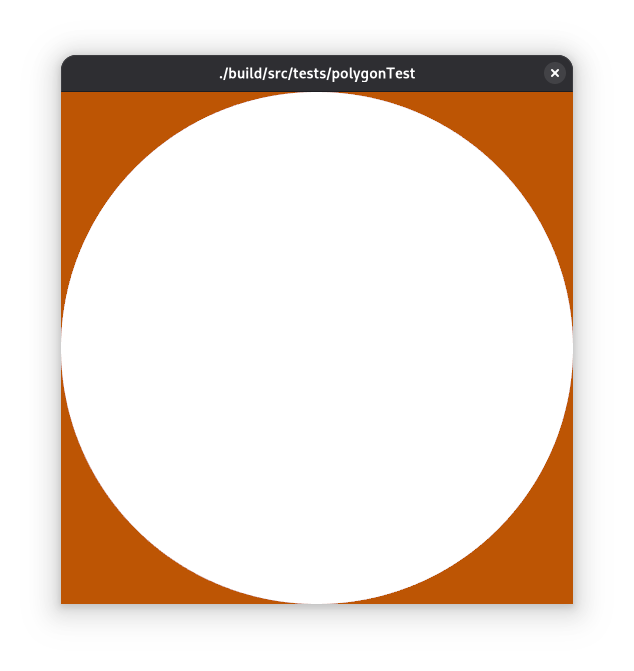
\includegraphics[width=1.0\textwidth]{figures/evidence/test_polygon_1000.png}
    \caption{Captura de pantalla de la prueba del polígono de 3 a 1000 vértices}
    \label{fig:test-polygon-1000}
\end{figure}


Utilizando los datos generados por la prueba se han creado varias gráficas que representan el rendimiento de la \textit{CPU} y la \textit{GPU} durante la ejecución. La primera gráfica representa el coste temporal que requiere crear los polígonos cuyos vértices aumentan progresivamente, desde \textbf{3} hasta \textbf{1000}, y la segunda y tercera gráfica representan la \textit{CPU} y la \textit{GPU} durante la renderización.

Observando la gráfica \ref{fig:polygon-graph-vertices}, se puede deducir a simple vista que es lineal. Con los resultados de diferentes medidas realizadas sobre estos datos en la tabla \ref{tbl:results-polygon-vertices} puede resaltarse:

\begin{itemize}

    \item Dado que $media > mediana > moda$, se deduce que los datos están sesgados positivamente y se acumulan hacia la izquierda de la gráfica.

    \item La desviación estándar y la varianza grandes indican que los datos difieren de la media bastante: que la varianza esté cerca de la mitad de la escala no es coincidencia, ya que la gráfica sigue una distribución lineal.

    \item El valor del \textit{IQR} confirma la anterior deducción: los datos en el medio de la gráfica tienen una dispersión del $3.43$, que es aproximado a la mitad de la escala.
    
    \item La correlación entre los datos de vértices y el tiempo de \textit{CPU} es cercana a $1$: siendo el crecimiento del número de vértices lineal, también lo sería el rendimiento.

\end{itemize}

\FloatBarrier

\begin{figure}[htp]
    \centering
    \includesvg[inkscapelatex=false, width=1.0\textwidth]{figures/graphs/polygon_graphs_vertices.svg}
    \caption{Gráfica que representa el rendimiento de la \textit{CPU} en la prueba del polígono durante su creación.}
    \label{fig:polygon-graph-vertices}
\end{figure}

\begin{table}[htp]
\centering

    % Esta primera línea define las columnas de la tabla. Los posibles tipos de columna son:
    % c: texto centrado
    % l: texto alineado a la izquierda
    % r: texto centrado a la derecha
    % p: columna de ancho fijo
    % Las columnas tienen ancho dinámico según la anchura máxima de los elementos que contengan.

    % Las columnas l/r/c no parten el texto en filas diferentes si éste es demasiado largo. Para ello, puede utilizar el tipo de columna de ancho fijo "p".
    
    % Las barras verticales | se usan para definir los bordes verticales de la tabla. Pruebe a eliminar algunas y observe qué ocurre.
    \begin{center}
    \begin{tabular}{ | l | l | }
        
        % A continuación van las filas de la tabla. En cada fila, las columnas se separan con el carácter &
        % Para terminar una fila se usa \\
        % Para incluir un borde horizontal entre filas se usa \hline
        
        % Cabecera con textos en negrita:
        \hline
        \textbf{Media: }  & 3.203347 \\
        \hline
        \textbf{Mediana} & 2.975000 \\
        \hline
        \textbf{Moda} & 2.518307 \\
        \hline
        \textbf{IQR} & 3.437500 \\
        \hline
        \textbf{Varianza} & 3.822103 \\
        \hline
        \textbf{Desviación estándar} & 1.955020 \\
        \hline
        \textbf{Covarianza (v)} & 561.004122 \\
        \hline
        \textbf{Correlación (v)} & 0.995537 \\
        \hline
        \textbf{Q1} & 1.5425 \\
        \hline
        \textbf{Q2} & 2.9750 \\
        \hline
        \textbf{Q2} & 4.9800 \\
        \hline
        
    \end{tabular} 
    \end{center}
    
    \caption{Resultados de la creación de vértices en la prueba del polígono}
    \label{tbl:results-polygon-vertices} 
\end{table}

\FloatBarrier

El par de gráficas \ref{fig:polygon-graphs-render} representan el rendimiento durante la renderización por parte de la \textit{GPU} y la \textit{CPU}. Las dos gráficas muestran un comportamiento logarítmico, aunque la primera se ajusta más a una función como $log(x)$ y la segunda como $log(log(x))$. Pueden observarse en los resultados de la \textit{GPU} \ref{tbl:results-polygon-render-gpu}:

\begin{itemize}

    \item La desviación estándar es muy pequeña respecto a los datos, lo que quiere decir que el \textit{jittering} es mínimo y los los datos no difieren mucho respecto a la media. 
    
    \item Dado que $media > mediana > moda$, se deduce que los datos están sesgados negativamente y se acumulan hacia la izquierda de la gráfica.
    
    \item La covarianza mayor a $0$ entre la \textit{CPU} y los vértices indica una dependencia entre los datos positiva.
    
    \item La correlación entre la \textit{CPU} y los vértices está entre $0$ y $1$, aunque acercándose a este último. Esto indica una relación positiva y lineal entre estas dos variables.
    
    \item Los cálculos de covarianza y correlación cercanos a $0$ entre la \textit{CPU} y la \textit{GPU} indican que los dos datos son independientes y no hay relación entre ellas.

\end{itemize}

\FloatBarrier
\begin{figure}[htp]
    \centering
    \includesvg[inkscapelatex=false, width=1.0\textwidth]{figures/graphs/polygon_graphs_render.svg}
    \caption{Gráficas que representan el rendimiento de la \textit{GPU} y la \textit{CPU} en la prueba del polígono durante la renderización.}
    \label{fig:polygon-graphs-render}
\end{figure}

\begin{table}[htp]
\centering

    % Esta primera línea define las columnas de la tabla. Los posibles tipos de columna son:
    % c: texto centrado
    % l: texto alineado a la izquierda
    % r: texto centrado a la derecha
    % p: columna de ancho fijo
    % Las columnas tienen ancho dinámico según la anchura máxima de los elementos que contengan.

    % Las columnas l/r/c no parten el texto en filas diferentes si éste es demasiado largo. Para ello, puede utilizar el tipo de columna de ancho fijo "p".
    
    % Las barras verticales | se usan para definir los bordes verticales de la tabla. Pruebe a eliminar algunas y observe qué ocurre.
    \begin{center}
    \begin{tabular}{ | l | l | }
        
        % A continuación van las filas de la tabla. En cada fila, las columnas se separan con el carácter &
        % Para terminar una fila se usa \\
        % Para incluir un borde horizontal entre filas se usa \hline
        
        % Cabecera con textos en negrita:
        \hline
        \textbf{Media: }  & 0.118084 \\
        \hline
        \textbf{Mediana} & 0.123392 \\
        \hline
        \textbf{Moda} & 0.134008 \\
        \hline
        \textbf{IQR} & 0.040960 \\
        \hline
        \textbf{Varianza} & 0.001664 \\
        \hline
        \textbf{Desviación estándar} & 0.040793 \\
        \hline
        \textbf{Covarianza (v)} & 7.548455 \\
        \hline
        \textbf{Correlación (v)} & 0.641963 \\
        \hline
        \textbf{Covarianza (GPU)} & 0.001354 \\
        \hline
        \textbf{Correlación (GPU)} & 0.759181 \\
        \hline
        \textbf{Q1} & 0.098304 \\
        \hline
        \textbf{Q2} & 0.123392 \\
        \hline
        \textbf{Q3} & 0.139264 \\
        \hline
        
    \end{tabular} 
    \end{center}
    
    \caption{Resultados de la renderización en la prueba del polígono: \textbf{GPU}}
    
    \label{tbl:results-polygon-render-gpu}
\end{table}
\FloatBarrier

Pueden observarse en los resultados de la \textit{CPU} \ref{tbl:results-polygon-render-cpu}:
\begin{itemize}

    \item La varianza y desviación típica son mayores que en las de la \textit{GPU} y son relativamente grandes respecto a la escala de los datos. Esto indica una alta dispersión en los resultados respecto a la media.

    \item El \textit{IQR} es cercano a 0, lo que indica una similitud entre cuartiles y, a su vez, mínima diferencia en los resultados.

    \item La covarianza entre la \textit{CPU} y los vértices indica una dependencia negativa entre estas dos variables: cuando aumentan los vértices, disminuye la duración de la \textit{CPU}.

    \item La correlación entre la \textit{CPU} y los vértices es cercana a $0$, lo que indica que existe independencia lineal entre estas dos variables.

    \item Los cálculos de covarianza y correlación cercanos a $0$ entre la \textit{CPU} y la \textit{GPU} indican que los dos datos son independientes y no hay relación entre ellas.

\end{itemize}

\FloatBarrier
\begin{table}[htp]
\centering

    % Esta primera línea define las columnas de la tabla. Los posibles tipos de columna son:
    % c: texto centrado
    % l: texto alineado a la izquierda
    % r: texto centrado a la derecha
    % p: columna de ancho fijo
    % Las columnas tienen ancho dinámico según la anchura máxima de los elementos que contengan.

    % Las columnas l/r/c no parten el texto en filas diferentes si éste es demasiado largo. Para ello, puede utilizar el tipo de columna de ancho fijo "p".
    
    % Las barras verticales | se usan para definir los bordes verticales de la tabla. Pruebe a eliminar algunas y observe qué ocurre.
    \begin{center}
    \begin{tabular}{ | l | l | }
        
        % A continuación van las filas de la tabla. En cada fila, las columnas se separan con el carácter &
        % Para terminar una fila se usa \\
        % Para incluir un borde horizontal entre filas se usa \hline
        
        % Cabecera con textos en negrita:
        \hline
        \textbf{Media}  & 0.132385 \\
        \hline
        \textbf{Mediana} & 0.130000 \\
        \hline
        \textbf{Moda} & 0.125230 \\
        \hline
        \textbf{IQR} & 0.010000 \\
        \hline
        \textbf{Varianza} & 0.001912 \\
        \hline
        \textbf{Desviación estándar} & 0.043723 \\
        \hline
        \textbf{Covarianza (v)} & 3.647974 \\
        \hline
        \textbf{Correlación (v)} & 0.289460 \\
        \hline
        \textbf{Covarianza (GPU)} & 0.001354 \\
        \hline
        \textbf{Correlación (GPU)} & 0.759181 \\
        \hline
        \textbf{Q1} & 0.13 \\
        \hline
        \textbf{Q2} & 0.13 \\
        \hline
        \textbf{Q3} & 0.14 \\
        \hline
        
    \end{tabular} 
    \end{center}
    
    \caption{Resultados de la renderización en la prueba del polígono: \textbf{CPU}}
    
    \label{tbl:results-polygon-render-cpu}
\end{table}

\section{Pruebas de rendimiento de animaciones} \label{sec:animation-performance-test}

Esta prueba se ha realizado con $2^{10}$ polígonos de \textbf{32} lados, o también llamados \textbf{icosidodecágonos}, desplegados por la pantalla. Para conseguir un escenario sencillo y previsible sobre la prueba, se decidió agrupar los polígonos en una matriz cuadrada y siempre la cantidad siendo $2^x$, donde $x$ es un número par con el objetivo de construir una matriz cuadrada de tamaño $2^{(x/2)}$ por $2^{(x/2)}$. Cada polígono obtiene sus coordenadas en función del número de polígonos a crear y de las dimensiones de la ventana. El diámetro de cada polígono se calcularía entonces como $\frac{1}{P}$, siendo $P$ el número de polígonos por fila o columna, para que cubran toda la ventana sin colisionar entre ellos, calculado como $P = 2^{\frac{M}{2}}$; Luego, considerando que en \textit{OpenGL} el origen de coordenadas está en el centro: $(x,y) = (-\frac{1}{2} + r + d \times i, \frac{1}{2} - (r + d \times j))$. El diámetro de cada polígono $d$ se calcula de manera inversamente proporcional a $P$: $d = \frac{1}{p}$. De esta forma, se coloca cada polígono en cada casilla de la matriz. Con estas coordenadas calculadas, puede llamarse a la función \textit{createNGonVertices} para crear el polígono regular.

\begin{algorithm}
\caption{Algoritmo de creación de polígonos en matriz cuadrada}\label{alg:polygon-matrix}
\begin{algorithmic}

\Require $M$ is \textbf{pair} and $N >0$ \Comment{$N$ is the number of vertices of each polygon}
\State $P \gets 2^{\frac{M}{2}}$ \Comment{$P$ is the number of polygons per row or column}
\State $d \gets \frac{1}{P}$ \Comment{$d$ is the diameter of each polygon}
\State $r \gets \frac{d}{2}$
\While{$j < P$}
    \While{$i < P$}
        \State $x \gets -\frac{1}{2} + r + d \times i$
        \State $y \gets \frac{1}{2} - (r + d \times j)$
        \newline
        \texttt{createNGonVertices($N$, $x$, $y$, $r$, \&(vertices[$P \times j + i$]))}
    \EndWhile
\EndWhile

\end{algorithmic}
\end{algorithm}

\subsection{Problemas encontrados}
En la prueba de animación, el principal problema residía en la naturaleza de la prueba a realizar; la cual consistía en reproducir una animación donde la mayor cantidad de polígonos actuaran a la vez en una misma escena, moviéndose al unísono, para comprobar cómo afectaría eso al rendimiento. Para poder representar todos estos polígonos a la vez y que fueran visibles, era necesario agruparlos correctamente y que no ocultasen unos a otros. Entonces, se calcularon las coordenadas de cada polígono como si de una matriz se tratase y cada figura un elemento de ella, con unos márgenes entre ellos para separarlos mínimamente. 

En esta prueba la posición en la que colocar las mediciones de tiempo era menos intuitiva. Ya que el objetivo principal era medir el rendimiento de la \textit{GPU}, se mide el tiempo entre fotogramas; asimismo, el rendimiento de la \textit{CPU} se mide en el mismo intervalo para poder comparar. También, fue útil medir el tiempo que tardaba la \textit{CPU} en crear todos los polígonos usados en la animación.

\subsection{Resultados}

Se muestra una captura de pantalla de la prueba de animación en funcionamiento \ref{fig:test-animation-1024}.

\begin{figure}[htp]
    \centering
    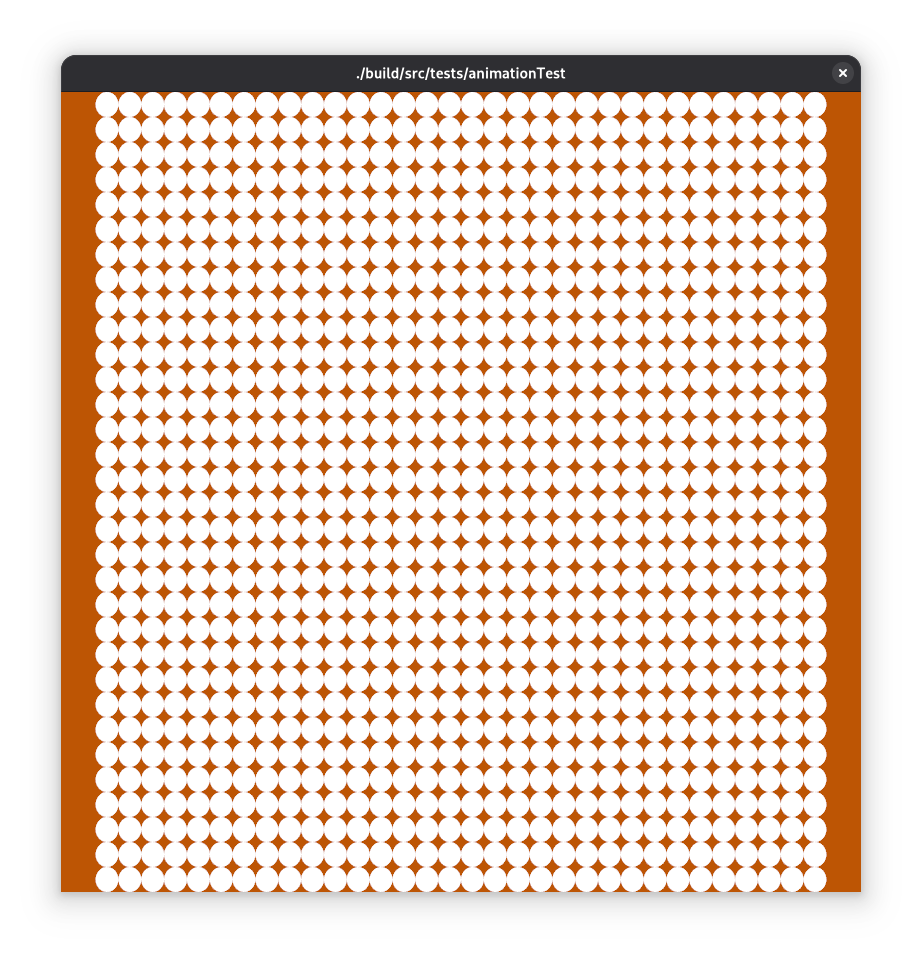
\includegraphics[width=1.0\textwidth]{figures/evidence/animation_1024.png}
    \caption{Captura de pantalla de la prueba de la animación de 1024 polígonos en una matriz cuadrada.}
    \label{fig:test-animation-1024}
\end{figure}

Los resultados de la \textit{CPU} \ref{fig:animation-graph-polygon} durante la creación de polígonos indican simetría y mínima dispersión:

\begin{itemize}

\item Dado que $media < mediana < moda$, se puede deducir que la distribución de los datos está sesgada negativamente y se acumulan ligeramente hacia la izquierda.

\item El \textit{IQR} calculado a partir de los cuartiles indica que la dispersión de los valores en la mitad de la gráfica tienen una dispersión de $0.03$, lo que es despreciable en esta escala.

\item Los valores de la variación y la desviación estándar son pequeños, lo que indica poca dispersión respecto a la media.

\end{itemize}

\FloatBarrier
\begin{figure}[htp]
    \centering
    \includesvg[inkscapelatex=false, width=1.0\textwidth]{figures/graphs/animation_graphs_polygon.svg}
    \caption{Gráfica que representa el rendimiento de la \textit{CPU} en la prueba de animación durante la creación de los polígonos.}
    \label{fig:animation-graph-polygon}
\end{figure}

\begin{table}[htp]
\centering

    % Esta primera línea define las columnas de la tabla. Los posibles tipos de columna son:
    % c: texto centrado
    % l: texto alineado a la izquierda
    % r: texto centrado a la derecha
    % p: columna de ancho fijo
    % Las columnas tienen ancho dinámico según la anchura máxima de los elementos que contengan.

    % Las columnas l/r/c no parten el texto en filas diferentes si éste es demasiado largo. Para ello, puede utilizar el tipo de columna de ancho fijo "p".
    
    % Las barras verticales | se usan para definir los bordes verticales de la tabla. Pruebe a eliminar algunas y observe qué ocurre.
    \begin{center}
    \begin{tabular}{ | l | l | }
        
        % A continuación van las filas de la tabla. En cada fila, las columnas se separan con el carácter &
        % Para terminar una fila se usa \\
        % Para incluir un borde horizontal entre filas se usa \hline
        
        % Cabecera con textos en negrita:
        \hline
        \textbf{Media: }  & 0.202725 \\
        \hline
        \textbf{Mediana} & 0.210000 \\
        \hline
        \textbf{Moda} & 0.224551 \\
        \hline
        \textbf{IQR} & 0.030000 \\
        \hline
        \textbf{Varianza} & 0.000965 \\
        \hline
        \textbf{Desviación estándar} & 0.031060 \\
        \hline
        \textbf{Q1} & 0.19 \\
        \hline
        \textbf{Q2} & 0.21 \\
        \hline
        \textbf{Q3} & 0.22 \\
        \hline
        
    \end{tabular} 
    \end{center}
    
    \caption{Resultados de la creación de polígonos en la prueba de animación (\textbf{CPU})}
    
    \label{table:results-animation-polygons}
\end{table}

\FloatBarrier

Pueden observarse en los resultados de la \textit{CPU}:
\begin{itemize}

    \item Dado que $media > mediana > moda$, se deduce que los datos están sesgados positivamente y se acumulan hacia la izquierda de la gráfica.

    \item Los valores de la varianza y la desviación típica son muy pequeños, lo que indica que los datos difieren muy ligeramente de la media.

    \item El \textit{IQR} con valor $0.047$ indica que la dispersión de los valores en la mitad de la gráfica es diminuta y su distribución es uniforme.

    \item La covarianza entre la \textit{CPU} y los vértices indica una dependencia negativa entre estas dos variables: cuando aumentan los vértices, disminuye la duración de la \textit{CPU}.

    \item La correlación entre la \textit{CPU} y los vértices es cercana a $0$, lo que indica que existe independencia lineal entre estas dos variables.

    \item Los cálculos de covarianza y correlación cercanos a $0$ entre la \textit{CPU} y la \textit{GPU} indican que los dos datos son independientes y no hay relación entre ellas.

\end{itemize}

La gráfica de la \textit{GPU} \ref{fig:animation-graphs-render} es interesante, ya que pueden distinguirse los distintos estados por los que pasa la animación: rotación, escala y traslación. Estos tres estados se ven reflejados en la gráfica con líneas en forma de \textit{zigzag} para la rotación, una línea recta para la traslación y una semiesfera para la escala (hacia abajo cuando se encoge y hacia arriba cuando se agranda). Sin embargo, la gráfica de la \textit{CPU} es constante, aunque con datos dispersos por la espera de sincronización entre los componentes.

\begin{figure}[htp]
    \centering
    \includesvg[inkscapelatex=false, width=1.0\textwidth]{figures/graphs/animation_graphs_render.svg}
    \caption{Gráficas que representan el rendimiento de la \textit{GPU} y la \textit{CPU} en la prueba de animación durante la renderización.}
    \label{fig:animation-graphs-render}
\end{figure}

\FloatBarrier

\begin{table}[htp]
\centering

    % Esta primera línea define las columnas de la tabla. Los posibles tipos de columna son:
    % c: texto centrado
    % l: texto alineado a la izquierda
    % r: texto centrado a la derecha
    % p: columna de ancho fijo
    % Las columnas tienen ancho dinámico según la anchura máxima de los elementos que contengan.

    % Las columnas l/r/c no parten el texto en filas diferentes si éste es demasiado largo. Para ello, puede utilizar el tipo de columna de ancho fijo "p".
    
    % Las barras verticales | se usan para definir los bordes verticales de la tabla. Pruebe a eliminar algunas y observe qué ocurre.
    \begin{center}
    \begin{tabular}{ | l | l | }
        
        % A continuación van las filas de la tabla. En cada fila, las columnas se separan con el carácter &
        % Para terminar una fila se usa \\
        % Para incluir un borde horizontal entre filas se usa \hline
        
        % Cabecera con textos en negrita:
        \hline
        \textbf{Media: }  & 0.206815 \\
        \hline
        \textbf{Mediana} & 0.192512 \\
        \hline
        \textbf{Moda} & 0.163906 \\
        \hline
        \textbf{IQR} & 0.047104 \\
        \hline
        \textbf{Varianza} & 0.002715 \\
        \hline
        \textbf{Desviación estándar} & 0.052101 \\
        \hline
        \textbf{Covarianza (GPU)} & 0.000971 \\
        \hline
        \textbf{Correlación (GPU)} & 0.419512 \\
        \hline
        \textbf{Q1} & 0.190464 \\
        \hline
        \textbf{Q2} & 0.192512 \\
        \hline
        \textbf{Q3} & 0.237568 \\
        \hline
        
    \end{tabular} 
    \end{center}
    
    \caption{Resultados de la renderización en la prueba del polígono: \textbf{GPU}}
    
    \label{table:results-animation-render-gpu}
\end{table}
\begin{table}[htp]
\centering

    % Esta primera línea define las columnas de la tabla. Los posibles tipos de columna son:
    % c: texto centrado
    % l: texto alineado a la izquierda
    % r: texto centrado a la derecha
    % p: columna de ancho fijo
    % Las columnas tienen ancho dinámico según la anchura máxima de los elementos que contengan.

    % Las columnas l/r/c no parten el texto en filas diferentes si éste es demasiado largo. Para ello, puede utilizar el tipo de columna de ancho fijo "p".
    
    % Las barras verticales | se usan para definir los bordes verticales de la tabla. Pruebe a eliminar algunas y observe qué ocurre.
    \begin{center}
    \begin{tabular}{ | l | l | }
        
        % A continuación van las filas de la tabla. En cada fila, las columnas se separan con el carácter &
        % Para terminar una fila se usa \\
        % Para incluir un borde horizontal entre filas se usa \hline
        
        % Cabecera con textos en negrita:
        \hline
        \textbf{Media}  & 0.177133 \\
        \hline
        \textbf{Mediana} & 0.170000 \\
        \hline
        \textbf{Moda} & 0.155733 \\
        \hline
        \textbf{IQR} & 0.000000 \\
        \hline
        \textbf{Varianza} & 0.001975 \\
        \hline
        \textbf{Desviación estándar} & 0.044440 \\
        \hline
        \textbf{Covarianza (GPU)} & 0.000971 \\
        \hline
        \textbf{Correlación (GPU)} & 0.419512 \\
        \hline
        \textbf{Q1} & 0.17 \\
        \hline
        \textbf{Q2} & 0.17 \\
        \hline
        \textbf{Q3} & 0.17 \\
        \hline
        
    \end{tabular} 
    \end{center}
    
    \caption{Resultados de la renderización en la prueba del polígono: \textbf{CPU}}
    
    \label{table:results-animation-render-cpu}
\end{table}

\section{Análisis de memoria} \label{sec:memory-analysis}
Utilizando la herramienta \textit{Valgrind}, especialmente la subherramienta \textit{Massif} \cite{webValgrindMassif}, se ha generado un informe del uso de memoria, especialmente la petición explícita de memoria (\textbf{pila} o \textit{heap)}, dentro de las dos pruebas. Las figuras \ref{fig:massif-visualizer-polygon} y \ref{fig:massif-visualizer-animation} representan el uso de memoria durante la prueba del polígono y animación, respectivamente, siendo el eje horizontal el tiempo y el vertical la memoria usada. Cada uno de los colores en la gráfica representa una función, mencionados en la leyenda, menos el color rojo que cubre al resto en la gráfica que representa el total. Se observa que el uso de memoria alcanza un techo y es constante desde entonces, alcanzando en las dos pruebas los \textbf{6MB} de memoria usados. También, las partes del programa que más memoria solicitaron fueron los \textit{drivers} de \textit{NVIDIA} de \textit{OpenGL}, con un uso insignificante frente a las funciones desarrolladas en el proyecto.

\begin{figure}[htp]
    \centering
    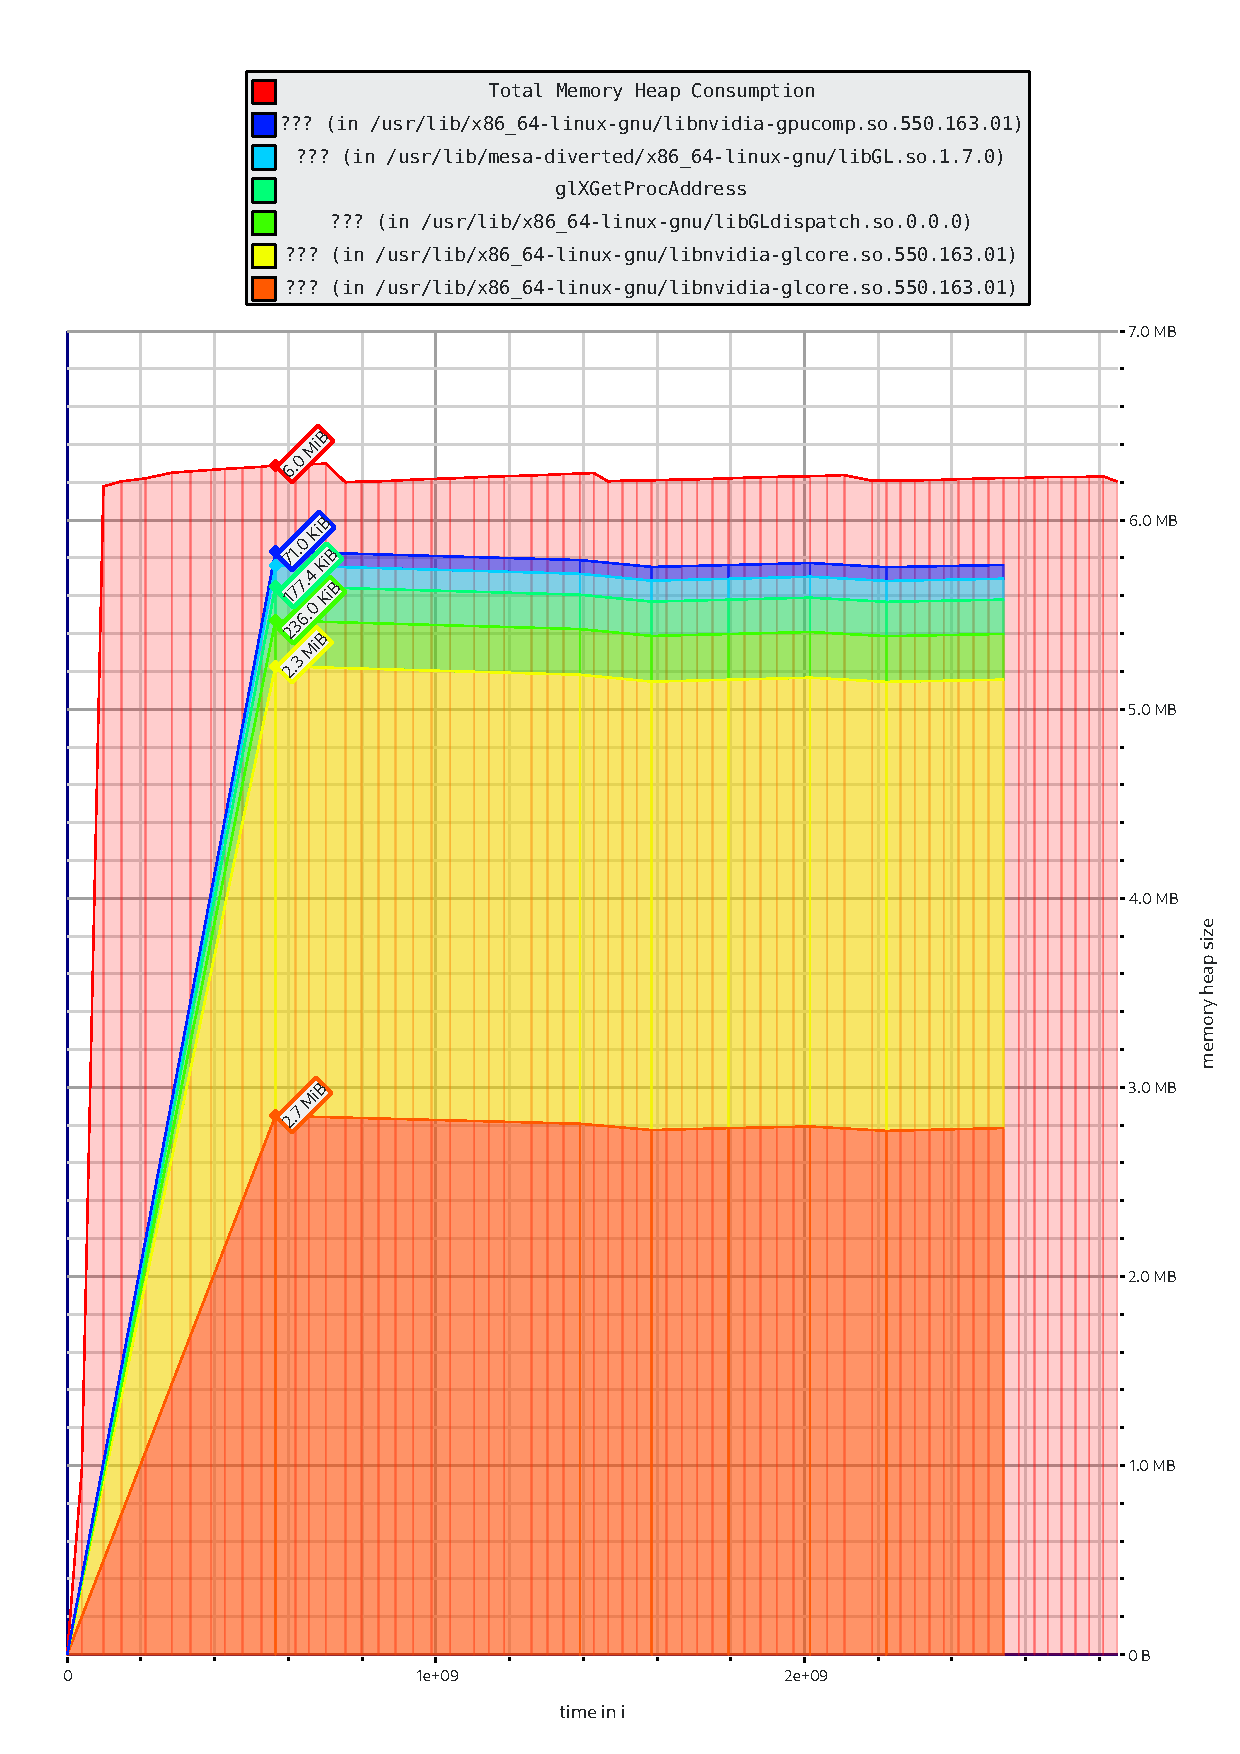
\includegraphics[width=1.0\textwidth]{figures/graphs/massif-visualizer-polygon.pdf}
    \caption{Gráfica que representa el uso de memoria en la prueba del polígono}
    \label{fig:massif-visualizer-polygon}
\end{figure}

\begin{figure}[htp]
    \centering
    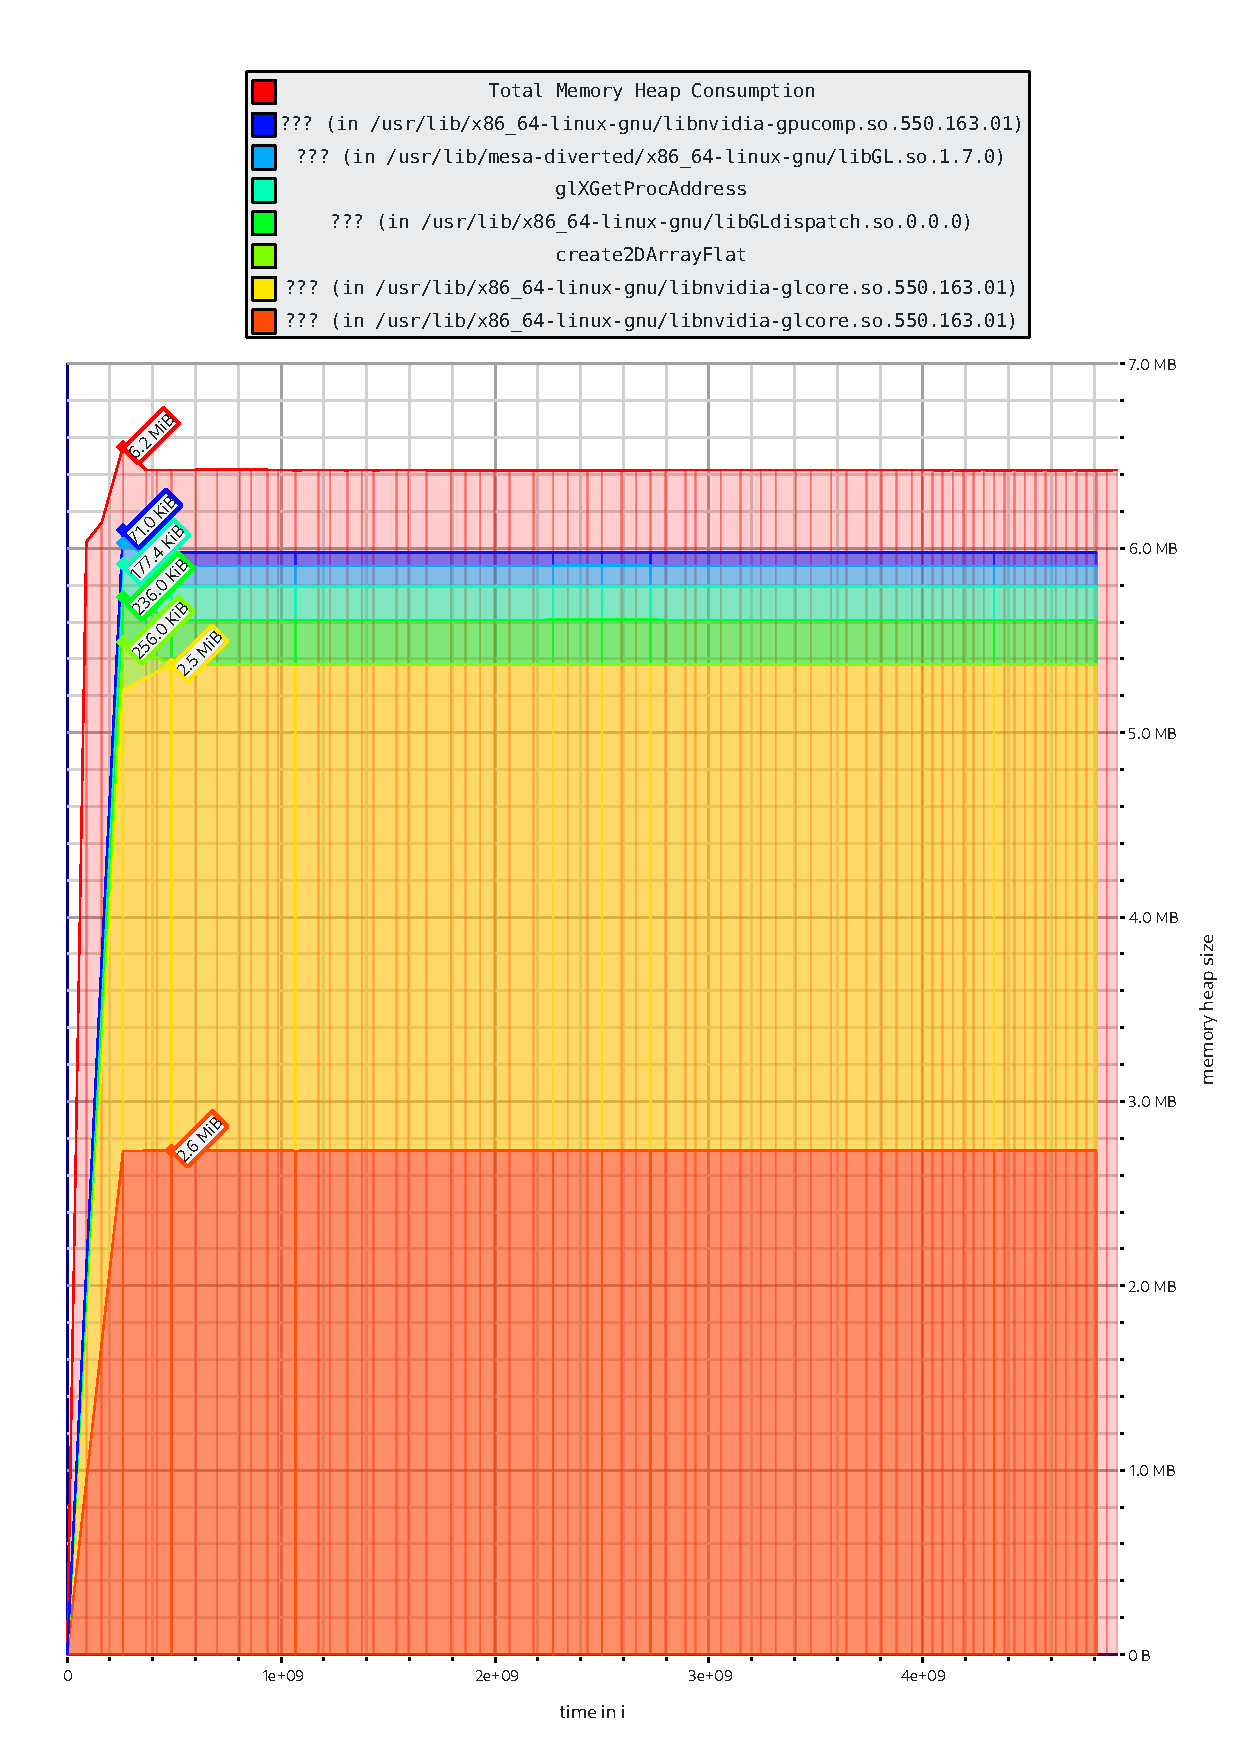
\includegraphics[width=1.0\textwidth]{figures/graphs/massif-visualizer-animation.pdf}
    \caption{Gráfica que representa el uso de memoria en la prueba de animación}
    \label{fig:massif-visualizer-animation}
\end{figure}

\section{Análisis de CPU} \label{sec:cpu-analysis}

\begin{table}[htp]
\centering

    % Esta primera línea define las columnas de la tabla. Los posibles tipos de columna son:
    % c: texto centrado
    % l: texto alineado a la izquierda
    % r: texto centrado a la derecha
    % p: columna de ancho fijo
    % Las columnas tienen ancho dinámico según la anchura máxima de los elementos que contengan.

    % Las columnas l/r/c no parten el texto en filas diferentes si éste es demasiado largo. Para ello, puede utilizar el tipo de columna de ancho fijo "p".
    
    % Las barras verticales | se usan para definir los bordes verticales de la tabla. Pruebe a eliminar algunas y observe qué ocurre.
    \begin{center}
    \begin{tabular}{ | l | l | l | }
        
        % A continuación van las filas de la tabla. En cada fila, las columnas se separan con el carácter &
        % Para terminar una fila se usa \\
        % Para incluir un borde horizontal entre filas se usa \hline
        
        % Cabecera con textos en negrita:
        \hline
        \textbf{Measure} & \textbf{Animation}  & \textbf{Polygon} \\
        \hline
        \textbf{Task clock (miliseconds)}  & 3,561 & 3,574 \\
        \hline
        \textbf{CPUs utilized}  & 0.367 & 0.915 \\
        \hline
        \textbf{Page faults} & 3,609  & 3,554\\
        \hline
        \textbf{Frequency (GHz)} & 3.187 & 3.268 \\
        \hline
        \textbf{Instructions per cycle} & 1.04 & 0.77 \\
        \hline
        \textbf{Branches per second} & 665.660 & 550.479 \\
        \hline
        \textbf{Branch misses percentage} & 1.21 & 1.14 \\
        \hline
        \textbf{Time elapsed (seconds)} & 9.7086 & 3.9050 \\
        \hline
        \textbf{Time user (seconds)} & 2.2427 & 1.1099 \\
        \hline
        \textbf{Time system (seconds)} & 1.3618 & 2.4674 \\
        \hline
        \textbf{Context switches} & 18,666 & 1,914 \\
        \hline
        \textbf{CPU migrations} & 331 & 26 \\
        \hline
        
    \end{tabular} 
    \end{center}
    
    \caption{Comparación de los resultados de la herramienta \textit{perf} durante la ejecución de las pruebas.}
    
    \label{tbl:perf-comparison}
\end{table}

Utilizando la herramienta \textit{perf}, con la subherramienta \textit{stat} \cite{webPerfStat}, se han recopilado datos del rendimiento de la \textit{CPU} durante la ejecución de las pruebas y se han presentado en la tabla \ref{tbl:perf-comparison}, donde para las pruebas de \textbf{animación} y \textbf{polígono} se toman diferentes \textbf{medidas}.

\begin{itemize}
    \item El tiempo tomado por ambas tareas es similar, aunque para la animación se haya utilizado un tercio de la cantidad de \textit{CPUs} que en polígono; lógico, ya que en la prueba de animación se divide la carga entre \textit{GPU} y \textit{CPU} más que en la prueba del polígono: el sistema de animaciones y algunas operaciones matriciales son tarea de la \textit{CPU}, mientras que la \textit{GPU} maneja operaciones de memoria y matriciales y renderizado.
    
    \item La frecuencia de la \textit{CPU} utilizada en las pruebas es \textit{3.5 GHz}, lo que concuerda con los resultados obtenidos.
    
    \item El \textit{IPC} o instrucciones por ciclo son mayores en la prueba de animación.
    
    \item Las migraciones de \textit{CPU} se relacionan con un traslado del proceso entre núcleos, semejante a los cambios de contexto, aunque este último se relaciona con el comportamiento del \textit{scheduler} o \textbf{planificador} del sistema operativo; ambos valores son más altos en la prueba de animación, debido a mayor número de bibliotecas involucradas y la necesidad de realizar múltiples tareas al mismo tiempo.

    \item El porcentaje de saltos fallidos es muy bajo, lo que indica una correcta predicción en la ejecución.

    \item La duración en segundos del usuario junto al sistema sí concuerda en la prueba del polígono, aunque no en la animación, ya que esta última no finaliza en cuanto se completa la renderización de los fotogramas.
    
\end{itemize}

\section{Conclusiones}
En este capítulo se han diseñado pruebas sobre los programas creados, midiendo el rendimiento y analizando los resultados. Se ha observado que, según el escenario, puede sufrir más el rendimiento de la \textit{CPU} o la \textit{GPU}: en la prueba de polígonos, era peor el rendimiento de la \textit{CPU}, y en la de animaciones, era peor el rendimiento de la gráfica.